\documentclass[t]{beamer}
\usepackage[utf8]{inputenc}

\usepackage{graphicx} 
\usepackage{booktabs} 
\usepackage{braket}
\usepackage{mathtools}
\usepackage{babel,blindtext}
\usepackage{mathrsfs,amsmath}
\usepackage{subcaption}
\usepackage{comment}
\usepackage[export]{adjustbox}

\newcommand{\R}{\mathbb{R}}
\newcommand{\Hy}{\mathbb{H}^3}
\newcommand{\Z}{\mathbb{Z}}
\newcommand{\ds}{\displaystyle}
\newcommand{\lh}{\mathcal{H}^1}
\newcommand{\lht}{\mathcal{H}^1(M_t)}
\newcommand{\sfc}{\overline{C^{\infty}_0}}
\newcommand{\Ima}{\text{Im}(H_2(M) \rightarrow H_2(M, \partial M))}
\newcommand{\fma}{\text{Im}(H^1_0(M) \rightarrow H^1(M))}
\newcommand{\va}{\varphi_{\delta}}
\newcommand{\st}{\Sigma_{\theta}}
\newcommand{\inj}{\text{inj}}
\newcommand{\vol}{\text{vol}}
\newcommand{\mt}{M_{\tau}}
\newcommand{\tn}{\textnormal}
\newcommand{\ok}{\Omega^k}
\newcommand{\okh}{\Omega^{k+1}}
\newcommand{\okl}{\Omega^{k-1}}
\newcommand{\okc}{\Omega^k_0}
\newcommand{\okhc}{\Omega^{k+1}_0}
\newcommand{\oklc}{\Omega^{k-1}_0}
\newcommand{\pc}{Poincar\'e }
\newcommand{\LL}{\mathcal{L}}
\newcommand{\sn}{\Sigma^{n-1}}
\newcommand{\Ric}{\textnormal{Ric}}
\newcommand{\Scal}{\textnormal{Scal}}


\mode<presentation>
{
  \usetheme{Madrid}      % or try Darmstadt, Madrid, Warsaw, ...
  \usecolortheme{default} % or try albatross, beaver, crane, ...
  \usefonttheme{default}  % or try serif, structurebold, ...
  \setbeamertemplate{navigation symbols}{}
  \setbeamertemplate{caption}[numbered]
} 
\title[]{Minimal Surface and Its Application to $3$-manifolds II                                                                                                                                                                                                                                                                                                                                                                                                                                                                                                                                                                                                                                                                                                                                                                                                                                                                                                                                                                                                                                                                                                                                                                                                                                                                                                                                                                                                                                                                                                                                                                                                                                                                                                                                                                                                                                                                                                                                                                                                                                                                                                                                                                                                                                                                                                                                                                                                                                                                                                                                                                                                                                                                                                                                                                                                                                  } 
\author{Xiaolong Hans Han} 
\institute[UIUC]
{
Toronto Geometric Analysis Seminar}
\date

\begin{document}

\begin{frame}
\titlepage 
\end{frame}

\begin{frame}
	\frametitle{Some remark for last time}
\end{frame}

\begin{frame}[t]
	\frametitle{Stability operator and stable minimal surface}
	Assume $\Sigma^{n-1}\subset M^n$ is minimal. Let $F$ be a normal variation, $F^T_t \equiv 0$. \textbf{The second variation} of $\Sigma$ is defined by
	\begin{equation}
		\ds \frac{d^2}{dt^2}\bigg|_{t=0} Vol(F(\Sigma, t)) =-\int_{\Sigma}\langle\ F_t, \LL F_t \rangle,
	\end{equation}
where $\LL$ is called stability or Jacobi operator. \par
\vspace{0.1in}
Assume $\Sigma$ has trivial normal bundle, then for a normal vector field $X= \nu N$, 
\begin{equation}
\LL \nu \coloneqq \Delta_{\Sigma} \nu +|A|^2 \nu +Ric_M(N,N) \nu
\end{equation}
\vspace{0.1in}
A minimal surface $\Sigma$ is called \textbf{stable} if
\begin{equation}
	\ds \frac{d^2}{dt^2}\bigg|_{t=0} Vol(F(\Sigma, t)) =-\int_{\Sigma}\langle\ F_t, \LL F_t \rangle \geq 0
\end{equation}
\end{frame}

\begin{frame}
		\frametitle{Morse index}
	We call $\lambda$ an eigenvalue of $\LL$ if 
	\begin{equation}
		\LL X +\lambda X=0
	\end{equation}
	The \textbf{Morse index} is defined to be the number of negative eigenvalues of $\LL$. \par 
	\vspace{0.1in}
	An index $1$ minimal surface and an index $5$ minimal surface:
	\vspace{1in}
	\begin{block}{Theorem, Urbano '90}
	Let $S$ be a compact orientable nontotally geodesic minimal surface in $S^3$. Then $\tn{ind}(M) \geq 5$, and the equality holds iff $M$ is a Clifford torus. 
	\end{block}
\end{frame}



\begin{frame}
	\frametitle{Examples of stable minimal surfaces}
	$2$-torus and hyperbolic helicoid (Biao Wang '19)
	\begin{figure}
		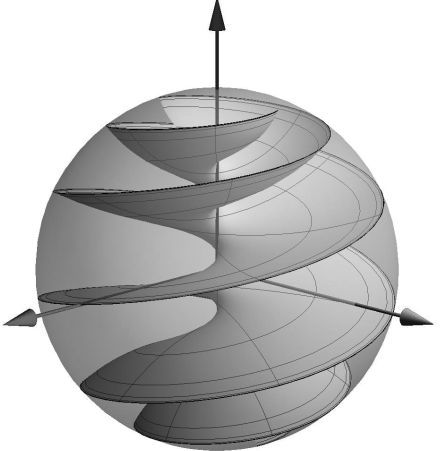
\includegraphics[scale=0.5, right]{HyperbolicHelicoid}
	\end{figure}

\vspace{0.8in}
Area minimizing surfaces in a homotopy class or homology class are stable. 
\end{frame}

\begin{frame}
	\frametitle{Complete stable surface in Euclidean space}
Existence of minimal surface with boundary, non-compact minimal surface like helicoid and catenoid. Stable non-compact min surfaces in $\Hy$. \par 
\begin{block}{Carmo-Peng '79, Schoen-Colbrie '80 (Bernstein 1917)}
A stable complete minimal surface in $\R^3$ is a plane. 
\end{block}

\end{frame}

\begin{frame}
	\frametitle{From ambient to submanifold and vice versa}
Suppose $\sn \subset M^n$ is a closed stable minimal hypersurface with trivial normal bundle. 
\begin{enumerate}
	\item Simons '68 : If $\Ric_M \geq 0$, then $\Sigma$ is totally geodesic and $\Ric_M(N,N)=0$ on $\Sigma$
	\item Schoen-Yau '79: If $\Scal_M >0$ and $n=3$, then $\Sigma$ is an $S^2$ or an $\R \mathbb{P}^2$ and 
	\begin{equation}
		\ds \int_{\Sigma} \Scal_M +|A|^2 \leq 8 \pi
	\end{equation}
Proof: 
\end{enumerate}
\vspace{1.2in}
Gao-Yau '86: Every closed $M^3$ admits a metric with negative Ricci. 
\end{frame}

\begin{comment}
\begin{frame}
\frametitle{Recent updates}
\begin{enumerate}
\item Nunes
\item Peng
\item Mical
\item Stern and Stern-Bray
\item Ben Lowe
\end{enumerate}
\end{frame}
\end{comment}

\begin{frame}
	\frametitle{Classical and geometric Dehn's Lemma}
	Dehn's lemma: If a Jordan curve on $\partial M^3$ compact is homotopically trivial, then it bounds an \textbf{embedded} disk. \par 
	Announced by Dehn 1910, a gap found Kneser '29, fixed by Papakyriakopoulos '57, simplified by Whitehead and Shapiro '57. 
\end{frame}

\begin{frame}
	\frametitle{Classical and geometric Dehn's Lemma}
Dehn's lemma: If a Jordan curve on $\partial M^3$ compact is homotopically trivial, then it bounds an \textbf{embedded} disk. \par 
Announced by Dehn 1910, a gap found Kneser '29, fixed by Papakyriakopoulos '57, simplified by Whitehead and Shapiro '57. 
\vfill
Geometric Dehn's Lemma, GDL (Meeks-Yau, '82): \par 
$M^3$ compact with $\partial M$ convex. If $\Gamma$ is a scc in $\partial M$ homotopically trivial in $M$, then: 
\begin{enumerate}
	\item $\exists f: D\rightarrow M$ of least-energy such that $f|_{\partial D}$ parameterizes $\Gamma$.
	\item $f$ above is $1-1$ and smooth immersion in $D^\mathrm{o}$. 
	\item $f$ is as regular as $\Gamma$ along $\partial D$. $\Gamma$ $C^2 \implies f$ an immersion. 
	\item If $f_1$ and $f_2$ are two such solutions and $f_1(D^\mathrm{o}) \cap f_2(D^\mathrm{o}) \neq \emptyset$, then $f_2=f_1$ up to conformal diffeomorphism reparameterization. 
\end{enumerate}
\end{frame}

\begin{frame}
	\frametitle{Cut and paste for Statement 4}
	Suppose that $D_1$, $D_2$ are two
	least-area embedded disks in $M$ with $\partial D_1 = \partial D_2 = \Gamma$, which intersect transversely at some interior point of the disks.
\end{frame}

\begin{frame}
	\frametitle{Outline for Statement 1 and 3}
\begin{enumerate}
	\item Extend $M$ to a homogeneously regular $\widetilde{M}$ without boundary.
	\vspace{2in} 
	\item Use Morrey '48 to get a least-energy map $f$.
	\item Use Osserman '70 and Gulliver '73 to conclude $f|_{\tn{int}(D)}$ is an immersion. Use Lewy '51 and Hildebrandt '69 to conclude the boundary regularity. 
\end{enumerate}
\end{frame}

\begin{frame}
	\frametitle{Proof of Statement 2}
Let $M^3$ be compact analytic. Suppose $D$ is the closed unit disk in the plane and $\gamma$ is an analytic curve on $\partial M$ and $f:D \rightarrow M$ is a least-area (energy) map with $f(\partial D) =f(D)\cap \partial M =\gamma$. Then $f$ is $1-1$. 
\vspace{0.1in}
\begin{enumerate}
	\item $f$ is an analytic immersion (Last slide + Morrey '48 for analyticity)
	\item $f$ is simplicial w.r.t. fixed triangulations of $D$ and $M$ (by Lojasiewicz '64). 
	\item two distinct analytic embedded disks (least-area w.r.t. boundary) have no interior intersections. 
	\vspace{0.5in}
	\item by barycentric subdivision, can assume the simplicial nbhd of $f(D)$ is a regular nbhd. 
	\begin{figure}
		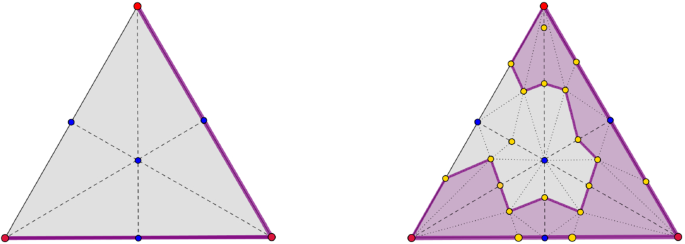
\includegraphics[scale=0.16]{BarycentricRegularNbhd}
	\end{figure}
\end{enumerate}

\end{frame}

\begin{frame}
	\frametitle{Refined tower construction using minimal surface}
	Construction of a tower for $f:D \rightarrow M$ to simplify the self-intersection for $f$:
	\par 
	$N_1$ a simplicial regular nbhd of $f(D)$. Restrict the range to get $f_1: D \rightarrow N_1$. If $N_1$ is not simply connected, take universal cover and lift to get $f_2$. 
\end{frame}

\begin{frame}
	\frametitle{A combinatorial upper bound on complexity}
	$T$ is the collection of open simplices and vertices. Let $c = \# T \times T$. Terminates $\leq c $ steps. \par
	\begin{block}{Lemma}
		If $S(f_i)=\{ (\sigma, \tau) \in T \times T|\sigma \neq \tau,  f(\sigma)=f(\tau)\}$, then $S(f_{i+1})$ is a proper subset of $S(f_i)$. Hence the tower construction terminates at finite steps. 
	\end{block}
\end{frame}

\begin{frame}
	
\end{frame}

\begin{comment}
\begin{frame}
	\frametitle{Heegaard surface}
	\begin{block}{Genus-$0$ splitting of $S^3$}
	\vspace{1.1in}
	\end{block}
	\begin{block}{Genus-$1$ splitting of $S^3$}
		\vspace{1.1in}
	\end{block}
\end{frame}
\end{comment}

\begin{frame}[t]
	\frametitle{Background and Motivation}
	\begin{block}{Mostow Rigidity and Effective Geometrization}
		When $M$ is finite-volume hyperbolic manifold with dim$\geq 3$, its geometry is determined by its topology. \par
	\end{block}
\end{frame}

\begin{frame}[t]
\frametitle{Norms on the Cohomology}
Measuring $H^1(M) \cong H_2(M)$\\
Thurston norm, $L^2$-norm, least area norm, $L^1$-norm, $L^{\infty}$-norm. 

\begin{block}{Thurston Norm} 
	For a compact irreducible $3$-manifold $M$, the Thurston norm of $\phi \in H^1(M; \mathbb{Z}) \cong H_2(M; \mathbb{Z})$ is defined by 
	\begin{center}
		$\chi_- (S)= \max\{0, -\chi(S)\}$
		$\| \phi \|_{Th}= \text{min}\{\chi_- (S)| \text{S is a properly embedded surface dual to } \phi \}$
	\end{center}
	When $M$ is closed hyperbolic, it is non-degenerate and a genuine norm.
\end{block}
\end{frame}

\begin{frame}[t]
	\frametitle{}
	\begin{block}{$L^2$ and $L^1$ Norm}
		
		\begin{center}
			$\ds |\alpha |_{L^2}^2 \coloneqq \int_M |\alpha(x)|^2 d \text{vol}_g(x) =\int_M \alpha \wedge *\alpha $
		\end{center}
		\begin{center}
			For $\phi \in H^1$, we have $\| \phi  \|_{L^2}= \ds \text{inf} \{ |\alpha |_{L^2}|\alpha \text{ represents } \phi \}$
		\end{center}
	\begin{center}
		$\ds |\alpha |_{L^1} \coloneqq \int_M |\alpha(x)| d \text{vol}_g(x) $
	\end{center}
	\end{block}
\begin{block}{Least Area Norm}
	For $\phi \in H^1$, let $\mathcal{F}_{\phi}$ be the collection of smooth maps $f: S \rightarrow M$ where $S$ is a closed oriented surface with $f_*([S])$ dual to $\phi$. The least area norm of $\phi$ is 
	\begin{center}
		$\|\phi \|_{LA}=\text{inf }\{\text{Area}(f(S))|f\in \mathcal{F}_{\phi}\}$
	\end{center} 
\end{block}
\end{frame}

\begin{frame}[t]
	\begin{block}{Theorem (Bergeron-Seng\"{u}n-Venkatesh 2015)}
		If $M$ is a finite of a fixed closed orientable hyperbolic $3$-manifold $M_0$, then we have \\
		\begin{center}
			$\frac{C_1}{\vol(M)} \|\cdot\|_{Th} \leq \|\cdot \|_{L^2}\leq C_2\|\cdot\|_{Th} \text{ on } H^1(M;\R)$
		\end{center}
		where $C_1$ and $C_2$ depend only on $M_0$. It generalizes Kronheimer-Mrowka. 
	\end{block}
\end{frame}

\begin{frame}[t]
	\begin{block}{Theorem (Bergeron-Seng\"{u}n-Venkatesh 2015)}
		If $M$ is a finite of a fixed closed orientable hyperbolic $3$-manifold $M_0$, then we have \\
		\begin{center}
			$\frac{C_1}{\vol(M)} \|\cdot\|_{Th} \leq \|\cdot \|_{L^2}\leq C_2\|\cdot\|_{Th} \text{ on } H^1(M;\R)$
		\end{center}
		where $C_1$ and $C_2$ depend only on $M_0$. It generalizes Kronheimer-Mrowka. 
	\end{block}
	\begin{block}{Theorem (Brock-Dunfield 2017), (Lin 2017)}
		For all closed orientable hyperbolic 3-manifolds M one has : 
		\begin{center}
			$\ds \frac{\pi}{\sqrt{\text{vol}(M)}} \| \cdot \|_{Th} \leq \| \cdot \|_{L^2} \leq \frac{10\pi}{\sqrt{\text{inj}}} \| \cdot \|_{Th}, \text{ on } H^1(M; \R) $
		\end{center} 
		(Lin 2017) uses the technique of Kronheimer-Mrowka to prove the LHS.
	\end{block}
	\begin{block}{Theorem (Stern 2019, Bray-Stern 2019)}
		Generalize the LHS to $3$-manifolds with boundary and reducible cases. 
	\end{block}
\end{frame}

\begin{comment}
\begin{frame}[t]
\frametitle{$H^1$ in Closed Hyperbolic $3$-manifold}
\begin{block}{Theorem (Brock-Dunfield 2017)}
For all closed orientable hyperbolic 3-manifolds M one has : 
\begin{center}
$\ds \frac{\pi}{\sqrt{\text{vol}(M)}} \| \cdot \|_{Th} \leq \| \cdot \|_{L^2} \leq \frac{10\pi}{\sqrt{\text{inj}}} \| \cdot \|_{Th}, \text{ on } H^1(M; \R) $
\end{center} 
It generalizes Kronheimer-Mrowka and Bergeron-Seng\"{u}n-Venkatesh.
\end{block}
\begin{block}{Remarks}
\begin{enumerate}
\item Can estimates on $\| \cdot \|_{Th}$ and hence  on $\| \cdot \|_{L^2}$.
\item  LHS can be approached by different techniques: harmonic map and Bochner technique for minimal surface in Bray and Stern, gauge theory in Kronheimer and Mrowka, Lin.. 
\item  RHS is much harder to prove.
\item  Not true for every geometry, e.g. $3$-torus.   
\end{enumerate}
\end{block}
\end{frame}
\end{comment}

\begin{frame}
	\frametitle{A Glance at the Noncompact Case}
	Finite-volume case also shares the rigidity and it is natural to wonder. 
	\begin{block}{inj$=0$}
		One immediate challenge: injectivity radius of $M$ is zero. We have to modify the inequality so that it can produce useful bounds on the $1$-form.  
	\end{block}
	\begin{block}{Thurston norm degenerate $H_2(M)$}
		The boundary-parallel torus has Thurston norm $0$ and area goes to $0$. 
	\end{block}
\end{frame}

\begin{comment}
\begin{frame}[t]
\frametitle{}
\begin{block}{$L^2$ norm may blow up for $H^1(M)$}
Consider $\phi$ dual to properly embedded thrice punctured sphere (or in general noncompact properly embedded surface). 
\end{block}
\end{frame}
\end{comment}

\begin{frame}[t]
	\frametitle{Solution is Surprisingly Simple!}
	\begin{block}{Only need to ask for $L^2$}
		The $L^2$ condition works extraordinarily well with Thurston norm and minimal surface theory. Denote $\lh$ the space of $L^2$ harmonic $1$-form. [Zucker, 1982 and Mazzeo-Phillips 1990] showed that $\lh  \cong \fma \cong \Ima$. 
	\end{block}
\end{frame}

\begin{comment}
\begin{frame}[t]
\frametitle{Solution is Surprisingly Simple!}
\begin{block}{Only need to ask for $L^2$}
The $L^2$ condition works extraordinarily well with Thurston norm and minimal surface theory. Denote $\lh$ the space of $L^2$ harmonic $1$-form. [Zucker, 1982 and Mazzeo-Phillips 1990] showed that $\lh \cong \fma \cong \Ima$. 
\end{block}
\frametitle{Topology and Geometry of $\lh$}
\begin{block}{Peripheral vs. Non-peripheral}
$H_2$ can be classified into peripheral and non-peripheral case. Peripheral classes are causing problems. Non-peripheral ones can be identified with those in Huang-Wang. 
\end{block}
\end{frame}
\end{comment}


\begin{frame}[t]
	\begin{block}{Lemma (H. '20):}
		\begin{enumerate}
			\item The Thurston norm is a genuine norm on $\lh$.
			\item The following estimates hold on $\lh$: 
			\begin{center}
				$\pi \| \cdot \|_{Th} \leq \| \cdot \|_{LA} \leq 2\pi \| \cdot \|_{Th}$
			\end{center}
		\end{enumerate}
		
	\end{block}
	Existence of LA surface established by Huang-Wang, Collin-Hauswirth-Mazet-Rosenberg is crucial. Apply arguments in Hass or Collin-Hauswirth-Mazet-Rosenberg for the estimates.  
\end{frame}

\begin{frame}[t]
	\frametitle{Compact Subdomain Suffices for the Inequality}
	\begin{block}{Theorem (H. '20):}
		For all finite-volume orientable hyperbolic $3$-manifolds $M$ one has 
		\begin{equation}
			\ds \frac{\pi}{\sqrt{\text{vol}(M)}} \| \cdot \|_{Th} \leq \| \cdot \|_{L^2} \leq \max\{\frac{10\pi}{\sqrt{\text{inj}(M_{\tau})}}, \frac{8\pi}{\text{inj}(M_{\tau})} \}  \| \cdot \|_{Th} \textnormal{ on } \lh
		\end{equation}
		$\tau$ is a constant explicitly computatble from $M$. 
	\end{block}
\end{frame}

\begin{comment}
\begin{frame}
\frametitle{Proof of Upper Bound}
\begin{block}{Tools from Brock-Dunfield}
Series expansion for harmonic functions in $\Hy$ (Minemura, Elstrodt-Grunewald-Mennicke) and a powerful inequality between $L^{\infty}$ and $L^2$. 
If $f: \Hy \rightarrow \R$ is harmonic, then $\exists a_{lm} \in \R$ such that 
\begin{center}
$f=\sum\limits_{l=0}^{\infty} \sum\limits_{m=-l}^{l} a_{lm} \Phi_{lm}$ 
\end{center}
and for $B=B_r(p)$ 
\begin{center}
$\ds |df_p| \leq \frac{1}{\sqrt{\nu (r)}} \|df \|_{L^2(B)}$

\end{center}
where $\nu(r)=6\pi (r+2r\text{csch}^2(r)-\coth(r)(r^2 \text{csch}^2(r)+1))$
\end{block}
\end{frame}
\end{comment}

\begin{frame}[t]
	\frametitle{Proof of Upper Bound}
	Counting duplicates when $M$ is lifted: \\
	\vspace{1.4in}
	\pc duality in closed vs. non-compact
\end{frame}

\begin{frame}[t]
	\frametitle{Proof of Upper Bound}
	For the closed case: Fix a surface $S$ dual to $\alpha$, and $\alpha$ is the harmonic representative of $\phi$. Thus we have
	\begin{align*}
		\|\alpha\|^2_{L^2} & =\int_M *\alpha \wedge \alpha =\int_S *\alpha \\
		&\leq \int_S |*\alpha| dA \leq \int_S \|\alpha\|_{L^\infty} dA  \\ &\leq \|\alpha\|_{L^\infty} Area(S) \leq 2\pi \|\alpha \|_{L^\infty} \|\alpha \|_{Th}
	\end{align*}
\end{frame}

\begin{frame}
	\begin{figure}
		\centering
		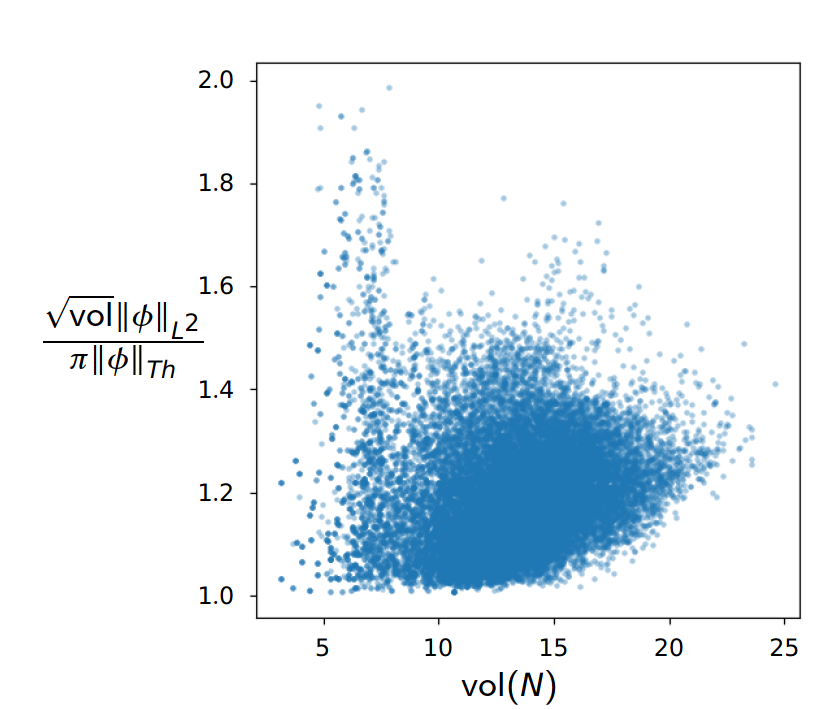
\includegraphics[width=.8\linewidth]{Dunfield-Hirani}
		\caption{Data from Dunfield-Hirani}	
	\end{figure}
\end{frame}

\begin{frame}[t]
	\frametitle{Sharpness for $M$ closed}
	Can it achieve $1$? 
	\begin{block}{Proposition (H. '20):}
		
		The LHS of the inequality in Brock-Dunfield will never be realized: 
		\begin{equation}
			\ds \frac{\pi}{\sqrt{\text{vol}(M)}} \| \cdot \|_{Th} < \| \cdot \|_{L^2}
		\end{equation}
	\end{block}
\end{frame}

\begin{comment}
\begin{frame}[t]
\frametitle{Sharpness for $M$ closed}
Can it achieve $1$? 
\begin{block}{Proposition (H. '20):}

The LHS of the inequality in Brock-Dunfield will never be realized: 
\begin{equation}
\ds \frac{\pi}{\sqrt{\text{vol}(M)}} \| \cdot \|_{Th} < \| \cdot \|_{L^2}
\end{equation}
\end{block}
\begin{block}{3 conditions to achieve equality}
\begin{enumerate}
\item Harmonic forms of constant length
\item Harmonic forms which realize its $L^1$-norm in the cohomological class
\item LA surfaces of genus $g$ with $Area=2\pi(g-1)$
\end{enumerate}
\end{block}
\end{frame}
\end{comment}

\begin{frame}[t]
	\frametitle{Proof of non-sharpness for Brock-Dunfield}
	\begin{block}{First Proof by Bochner technique (Inspired by Stern)}
		Let $\alpha$ be a harmonic $1$-form with constant length $c$, By Bochner formula, 
		\begin{center}
			$ | \nabla \alpha |^2=2|\alpha|^2=2c^2$
		\end{center}
		The second fundamental form on $S$ is 
		\begin{center}
			$\ds \sigma_S =\frac{\nabla \alpha}{|\alpha|} \Big\vert_S  $
		\end{center}
		which implies that 
		\begin{center}
			$\ds |\sigma_S|^2=2 $
		\end{center} 
		Contradicts the property of holomorphic quadratic differential. 	
	\end{block}
	
\end{frame}

\begin{frame}[t]
	\frametitle{Second proof based on Wolf-Wu}
	\begin{block}{Wolf-Wu: Geometric folitation}
		Locally geometric $1$-parameter family of closed minimal surface: if $\exists$ a closed surface $S$, $\epsilon >0$, an embedding: 
		\begin{equation}
			h: (-\epsilon, \epsilon) \times S \rightarrow M
		\end{equation}
		$\forall p\in S$, $f(t, p)\coloneqq \langle (h_t)_*(\partial_t), \nu \rangle |_{t=0}$ only depends on the principal curvature of $S$ at p.
		
	\end{block}
\end{frame}

\begin{comment}
\begin{enumerate}
\item $h$ is $C^2$
\item $\forall t$, the leaf $h_t$ is a minimal surface
\item $f(0, \cdot) : S\rightarrow \R$ is not identically $0$. 
\end{enumerate}
\end{comment}

\begin{frame}
	\frametitle{Geometric foliation and harmonic forms of constant length}
	\begin{enumerate}
		\item Harmonic form with constant length gives a foliation by minimal surface (fibered over $S^1$) with orthogonal geodesic flow. Particular case of Wolf-Wu. 
		\item Theorem (Zeghib, '83): There is no smooth vector fields on a closed hyperbolic $3$-manifold where all flow lines are geodesic. 
	\end{enumerate}
	\vspace{1in}
	Non-sharpness in the non-compact case is easier to prove, thanks to Mazzeo-Phillips, on asymptotic of harmonic forms near infinity. 
\end{frame}

\begin{frame}
	\begin{block}{A conjecture from Brock-Dunfield}
		Let $M_j$ be a sequence of orientable closed hyperbolic $3$-manifolds, converging geometrically to $M$. Then the 
		\begin{equation}
			\sup_{H^1(M_j)} \frac{\|\cdot \|_{L^2}}{\|\cdot \|_{Th}} \sim \mathcal{O}\left({\sqrt{-\log(\inj(M_j))}} \right)	
		\end{equation}
		\begin{figure}
			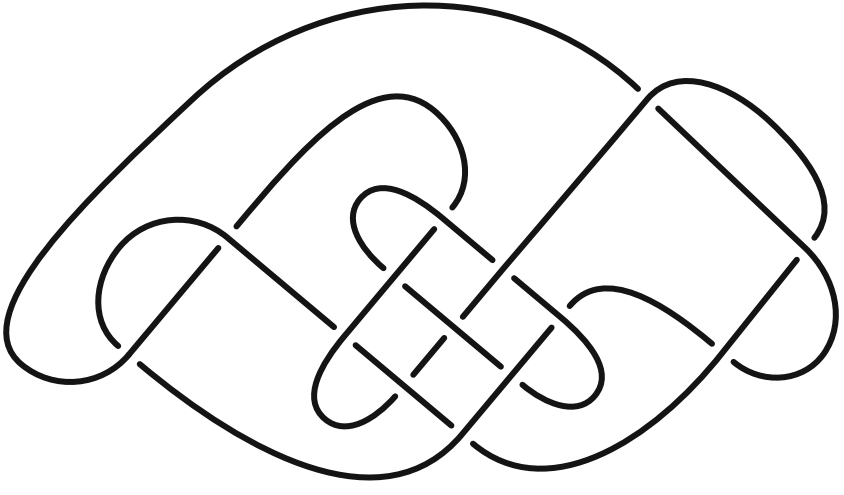
\includegraphics[scale=0.2]{L14n21792}
			\caption{L14n21792}
		\end{figure}
		$M_j$ is obtained from $M$ by particular Dehn fillings. 
	\end{block}
	Natural questions: one cusp? More than two cusps?
\end{frame}

\begin{frame}[t]
	\begin{block}{Theorem, H' 21}
		Let $M_j$ be a sequence of orientable closed hyperbolic $3$-manifolds, converging geometrically to $M$ with one cusp. Then for $j$ large enough,
		\begin{equation}
			\sup_{H^1(M_j)} \frac{\|\cdot \|_{L^2}}{\|\cdot \|_{Th}} < C
		\end{equation}
		where $C$ depends on $M$. 
	\end{block}
For $n$ cusps, this is generic. 
Geometric convergence vs. Dehn fillings: 
\end{frame}

\begin{frame}[t]
	\textbf{Outline of proof}
	(for large $j$)
	\begin{enumerate}
		\item Use Hatcher '82 to conclude $H_2(M_j)$ all come from the closed non-peripheral surfaces from $M$, $Im$. Use Agol '01 to control the topological complexity;
		\vfill
		\item Use barrier surface arguments to argue no deep disk, as in Wang '12, Huang-Wang '18, Hass '15, Mazet-Rosenberg '20. Use $k$-bi-Lipshitz diffeomorphism between thick part of $M_j$ and $M$ to argue no deep annulus, by the work of Futer-Purcell-Schleimer '19 (based on Bromberg-Brock 04, Hodgson-Kerckhoff '02 ) and Huang-Wang '17;
		\vfill
		\item Modify Brock-Dunfield, replace $\inj(M_j)$ by $\epsilon(M)$. 
		\vfill
	\end{enumerate}
\end{frame}

\begin{frame}
\huge	Thanks to the organizers and the audiences!
\end{frame}




  
\end{document}=